\documentclass[conference]{IEEEtran}
\IEEEoverridecommandlockouts

\usepackage{cite}
\usepackage{amsmath,amssymb,amsfonts}
\usepackage{algorithmic}
\usepackage{graphicx}
\usepackage{textcomp}
\usepackage{xcolor}
\usepackage{booktabs}
\usepackage{multirow}
\usepackage{array}
\usepackage{microtype}
\usepackage[colorlinks=true, linkcolor=black, citecolor=black, urlcolor=black]{hyperref}
\usepackage{tikz}
\usetikzlibrary{shapes,arrows,positioning,fit,calc}
\usepackage{pgfplots}
\pgfplotsset{compat=1.18}

\def\BibTeX{{\rm B\kern-.05em{\sc i\kern-.025em b}\kern-.08em
    T\kern-.1667em\lower.7ex\hbox{E}\kern-.125emX}}

%================== DOCUMENT ==================%
\begin{document}

\title{A Hybrid Deep Learning and Monte Carlo Framework for European Option Pricing\\}

\author{
\IEEEauthorblockN{Prahallad Padhan}
\IEEEauthorblockA{\textit{Department of Computing Technologies} \\
\textit{SRM Institute of Science}\\
\textit{and Technology}\\
Chennai, India \\
pp8509@srmist.edu.in}
\and

\IEEEauthorblockN{Shivansh Srivastava}
\IEEEauthorblockA{\textit{Department of Computing Technologies} \\
\textit{SRM Institute of Science}\\
\textit{and Technology}\\
Chennai, India \\
ss1420@srmist.edu.in}
\and

\IEEEauthorblockN{Mrs. Vathana D}
\IEEEauthorblockA{\textit{Department of Computing Technologies} \\
\textit{SRM Institute of Science}\\
\textit{and Technology}\\
Chennai, India \\
vathana.d@ktr.srmuniv.ac.in}
}

\maketitle

%================== ABSTRACT ==================%
\begin{abstract}
Pricing options correctly is at the heart of financial risk management, yet the classical Black--Scholes framework relies on idealized assumptions---constant volatility, log-normal returns---that rarely hold in practice. This paper presents OptionQuant, an end-to-end platform that brings together Monte Carlo simulation, deep learning, and modern quantitative techniques to price European call options and deliver actionable risk analytics. At its core, the system pairs a high-performance Monte Carlo engine (supporting four variance reduction strategies) with a deep neural network trained on simulated pricing data, a Physics-Informed Neural Network that bakes the Black--Scholes PDE directly into its loss function, an LSTM-based volatility forecaster, and a Transformer model for implied volatility surfaces. Beyond pricing, the platform incorporates reinforcement learning agents for dynamic hedging, Bayesian uncertainty quantification, Hidden Markov Model regime detection, Merton jump diffusion and Heston stochastic volatility models, arbitrage scanning, portfolio-level Value-at-Risk with stress testing, and SHAP-based explainability---all exposed through 48 production-grade REST endpoints with real-time WebSocket support. Trained on $M = 50{,}000$ synthetic samples generated from $N = 100{,}000$ GBM paths per sample, the proposed deep learning model achieves an MSE of $8.1 \times 10^{-6}$, an RMSE of $0.0028 \pm 0.0001$, an MAE of $0.0015 \pm 0.0001$, and an $R^2$ of 0.9997 relative to the analytical Black--Scholes solution, with errors distributed near-uniformly across moneyness buckets. Crucially, a single forward pass completes in just 0.8\,ms---roughly $150\times$ faster than a 100{,}000-path Monte Carlo run and only 60\% slower than the closed-form Black--Scholes evaluation---making real-time pricing entirely feasible. Because the training labels are themselves Monte Carlo estimates under constant-parameter GBM, the results should be interpreted as showing that a neural network can faithfully reproduce the simulation-based pricing surface rather than as evidence of superiority over the analytical formula. Nonetheless, the findings demonstrate that a well-designed hybrid of stochastic simulation and data-driven learning can match analytical accuracy at a fraction of the computational cost, making the approach practical for high-frequency trading, institutional risk management, and large-scale portfolio evaluation.
\end{abstract}

\begin{IEEEkeywords}
Option Pricing, Monte Carlo Simulation, Black--Scholes Model, Deep Learning, Physics-Informed Neural Networks, Reinforcement Learning, Volatility Surface, LSTM, Transformer, Geometric Brownian Motion, Computational Finance, Stochastic Volatility, Risk Analytics, Uncertainty Quantification
\end{IEEEkeywords}

% ================================================================
\section{Introduction}
% ================================================================

Pricing financial derivatives---options in particular---remains one of the central challenges in quantitative finance. When an option is priced accurately, it helps traders manage risk, build efficient portfolios, and make better-informed decisions. Among the many types of derivatives, European options receive the most attention in both academic research and industry practice, largely because they lend themselves to clean analytical treatment. The celebrated Black--Scholes model~\cite{b1} gives a closed-form price for these options by assuming constant volatility, no transaction costs, log-normal asset returns, and the ability to trade continuously.

These assumptions were ground-breaking in the 1970s, but decades of empirical evidence have revealed their shortcomings. Volatility clusters, heavy-tailed return distributions, and abrupt regime shifts are commonplace in real markets~\cite{b2,b3}. When such phenomena are ignored, purely analytical prices can be misleading. This is why practitioners routinely turn to Monte Carlo simulation, which can accommodate almost any stochastic process by generating a large number of random asset-price paths and averaging the discounted payoffs~\cite{b4}. The trade-off, however, is computational: high accuracy demands hundreds of thousands of simulated paths, and convergence is slow, scaling only as $1/\sqrt{N}$.

Over the past several years, advances in deep learning and GPU hardware have opened a different door. Neural networks---including Long Short-Term Memory (LSTM) architectures, Transformers, and Physics-Informed Neural Networks (PINNs)---can learn the nonlinear mapping from option parameters to prices by studying training data, rather than solving differential equations from scratch each time~\cite{b5,b6}. Once trained, they return answers in milliseconds. At the same time, modern practitioners expect more than just a price: they want interpretable explanations, uncertainty bands, regime-aware signals, and real-time hedging recommendations.

Motivated by these needs, we developed \textbf{OptionQuant}---a fully integrated, AI-powered option pricing and risk analytics platform. Rather than treating analytical methods, simulation, and deep learning as isolated tools, we combine them inside a single production-grade system. The main contributions of this work can be summarised as follows:

\begin{itemize}
    \item A high-performance Monte Carlo engine with four variance reduction strategies (antithetic variates, control variates, stratified sampling, and importance sampling), backed by optional GPU acceleration.
    \item A suite of deep learning models---a feedforward regression network for pricing, an LSTM for volatility forecasting, and a Transformer for implied volatility surfaces---all trained on Monte Carlo-generated data.
    \item A Physics-Informed Neural Network that embeds the Black--Scholes PDE and no-arbitrage constraints directly into its loss, ensuring physically consistent predictions.
    \item Reinforcement learning agents (DQN and PPO) for dynamic delta hedging, plus Bayesian uncertainty quantification, HMM regime detection, Merton jump diffusion, Heston stochastic volatility, arbitrage scanning, and portfolio-level risk analytics.
    \item A complete system architecture---48 REST endpoints, WebSocket streaming, JWT authentication, an interactive dashboard, Kubernetes manifests, and Prometheus monitoring---designed for institutional deployment.
    \item A thorough comparative evaluation against the analytical Black--Scholes solution using MSE, RMSE, MAE, and wall-clock timing.
\end{itemize}

The rest of the paper is laid out as follows. Section~\ref{sec:related} surveys the relevant literature. Section~\ref{sec:math} covers the mathematical foundations. Section~\ref{sec:methodology} walks through our methodology and system design. Section~\ref{sec:experiments} presents the experimental results, and Section~\ref{sec:conclusion} wraps up with conclusions and directions for future work.

% ================================================================
\section{Related Work}\label{sec:related}
% ================================================================

The option pricing literature spans analytical, numerical, and, more recently, data-driven approaches. We briefly review the strands most relevant to our work.

\subsection{Monte Carlo Simulation Methods}

Monte Carlo methods have long been a workhorse for derivative valuation because they can handle payoff structures and stochastic dynamics that elude closed-form treatment. Hui~et~al.~\cite{b7} compared Asian and European option pricing via Monte Carlo and highlighted practical differences in estimation stability between the two. Working on a less common asset-price model, Hartinger and Predota~\cite{b8} showed that quasi-Monte Carlo sequences and importance sampling can significantly speed up convergence for Asian options under hyperbolic dynamics.

Several authors have also applied Monte Carlo outside the option-pricing setting. Siddiaui and Patil~\cite{b9} used it for equity valuation, while Xiang~et~al.~\cite{b10} and Dewi~et~al.~\cite{b11} employed GBM-based simulations to forecast stock prices in developed and emerging markets, respectively. All of these studies underline the flexibility of simulation-based methods; at the same time, they share a common limitation---none of them benchmark their results against a machine learning alternative, leaving open the question of whether data-driven models could achieve comparable accuracy at lower computational cost.

Glasserman's textbook~\cite{b4} remains the definitive reference for variance reduction techniques---antithetic variates, control variates, stratified sampling, and importance sampling---that we adopt in our Monte Carlo engine.

\subsection{Extensions to the Black--Scholes Framework}

Researchers have tried to relax the restrictive assumptions of the original Black--Scholes model in several ways. Zhang and Wang~\cite{b12} replaced crisp parameters with fuzzy numbers to capture coefficient uncertainty. Youness~et~al.~\cite{b13} reformulated the equation with fractional derivatives to introduce memory effects, and Sun~\cite{b14} combined the model with genetic algorithms for patent valuation. Deng and Xi~\cite{b16} explored reset option pricing under fractional Brownian motion, departing from the Markovian assumption.

Two extensions are particularly relevant to our platform. Heston~\cite{b18} introduced a stochastic volatility model whose mean-reverting variance process generates the implied-volatility smiles observed in practice. Merton~\cite{b2} added Poisson-driven jumps to GBM, accounting for the sudden price discontinuities that a pure diffusion model cannot reproduce. Both models are implemented and compared in our system.

\subsection{Machine Learning and Deep Learning Approaches}

The idea of using neural networks for option pricing dates back to Hutchinson, Lo, and Poggio~\cite{b25}, who showed in 1994 that a shallow network trained on simulated Black--Scholes data could learn the pricing function to high accuracy---an early demonstration that data-driven models can approximate complex financial mappings. More recently, Ruf and Wang~\cite{b26} provided a comprehensive survey of neural-network approaches to option pricing, cataloguing architectures, training strategies, and open challenges across more than 150 studies.

With the rise of affordable GPU computing, deep learning has gained further traction in quantitative finance. Patil~et~al.~\cite{b15} demonstrated that coupling an LSTM with GBM improved stock-price forecasts, though their focus was on equity prices rather than option pricing. Dossatayev~\cite{b17} applied convolutional neural networks directly to option price forecasting and achieved promising results, but did not compare them against a Black--Scholes baseline.

On the methodological side, Raissi~et~al.~\cite{b19} pioneered Physics-Informed Neural Networks (PINNs), which embed the governing PDE of a physical system into the training loss and thereby enforce structural consistency. Buehler~et~al.~\cite{b20} and Cao~et~al.~\cite{b21} explored reinforcement learning for hedging derivatives, showing that learned policies can outperform classical delta hedging in the presence of transaction costs. Lundberg and Lee~\cite{b22} introduced SHAP values, a model-agnostic method for local feature attribution that has since become the de~facto standard for explaining black-box predictions.

\subsection{Research Gap}

Looking across this body of work, a clear pattern emerges: most studies focus on one technique in isolation---better simulation, a smarter neural network, or a novel stochastic model---without systematically comparing pricing accuracy, computational cost, and interpretability within a single, integrated system. Our platform addresses this gap by unifying analytical pricing, Monte Carlo simulation (with four variance reduction methods and GPU support), multiple deep learning architectures (feedforward, LSTM, PINNs, Transformer), reinforcement learning hedging, Bayesian uncertainty quantification, HMM regime detection, arbitrage scanning, and SHAP-based explainability under one roof. Table~\ref{tab:comparison_existing} summarises how existing work compares with our approach.

\begin{table}[htbp]
\caption{Positioning of the Present Study Among Related Work}
\label{tab:comparison_existing}
\centering
\small
\setlength{\tabcolsep}{3pt}
\renewcommand{\arraystretch}{0.95}
\resizebox{\columnwidth}{!}{
\begin{tabular}{p{1.6cm}p{1.4cm}p{1.9cm}p{2.3cm}}
\toprule
\textbf{Author} & \textbf{Method} & \textbf{Focus} & \textbf{Limitation} \\
\midrule
Hui et al.~\cite{b7} & MC & Asian vs European & No ML comparison \\
Hartinger~\cite{b8} & Quasi-MC & Asian options & Complex assumptions \\
Zhang \& Wang~\cite{b12} & Fuzzy BS & Parameter uncertainty & No benchmarking \\
Patil et al.~\cite{b15} & LSTM+GBM & Stock forecasting & Not option pricing \\
Dossatayev~\cite{b17} & Deep Learning & Option forecasting & No BS comparison \\
Raissi et al.~\cite{b19} & PINNs & PDE solving & Not finance-specific \\
Buehler et al.~\cite{b20} & Deep RL & Hedging & No pricing comparison \\
Hutchinson~\cite{b25} & Shallow NN & BS learning & Single architecture \\
Ruf \& Wang~\cite{b26} & Survey & NN pricing & No new model \\
\textbf{Proposed} & \textbf{Hybrid} & \textbf{Full platform} & \textbf{Integrated system} \\
\bottomrule
\end{tabular}
}
\end{table}


% ================================================================
\section{Mathematical Background}\label{sec:math}
% ================================================================

We briefly review the mathematical machinery that our platform builds upon; readers already familiar with these models may wish to skip to Section~\ref{sec:methodology}.

\subsection{Black--Scholes Model}

The Black--Scholes framework~\cite{b1} assumes that the underlying asset price follows a Geometric Brownian Motion (GBM):
\begin{equation}
    dS_t = \mu S_t \, dt + \sigma S_t \, dW_t
\end{equation}
where $S_t$ represents the asset price at time $t$, $\mu$ is the drift rate, $\sigma$ is the volatility, and $W_t$ denotes a standard Wiener process.

Under the risk-neutral measure, the drift term $\mu$ is replaced by the risk-free rate $r$:
\begin{equation}
    dS_t = r S_t \, dt + \sigma S_t \, dW_t
\end{equation}

The closed-form solution for a European call option is:
\begin{equation}
    C(S_0, T) = S_0 N(d_1) - K e^{-rT} N(d_2)
\end{equation}
where
\begin{equation}
    d_1 = \frac{\ln\left(\frac{S_0}{K}\right) + \left(r + \frac{1}{2}\sigma^2\right)T}{\sigma\sqrt{T}}, \quad d_2 = d_1 - \sigma\sqrt{T}
\end{equation}

Here, $S_0$ is the initial stock price, $K$ is the strike price, $T$ is the time to maturity, $r$ is the risk-free interest rate, $\sigma$ is volatility, and $N(\cdot)$ denotes the cumulative distribution function of the standard normal distribution. The analytical Greeks are computed as:
\begin{align}
    \Delta &= N(d_1), \quad \Gamma = \frac{n(d_1)}{S_0 \sigma \sqrt{T}} \\
    \mathcal{V} &= S_0 n(d_1) \sqrt{T}, \quad \Theta = -\frac{S_0 n(d_1) \sigma}{2\sqrt{T}} - rKe^{-rT}N(d_2) \\
    \rho &= KTe^{-rT}N(d_2)
\end{align}
where $n(\cdot)$ is the standard normal density function.

\subsection{Geometric Brownian Motion Solution}

Integrating the risk-neutral SDE yields the well-known log-normal solution:
\begin{equation}\label{eq:gbm_solution}
    S_T = S_0 \exp\left[\left(r - \frac{1}{2}\sigma^2\right)T + \sigma\sqrt{T}\,Z\right]
\end{equation}
where $Z \sim \mathcal{N}(0,1)$ is a standard normal random variable.

\subsection{Monte Carlo Simulation for Option Pricing}

The idea behind Monte Carlo pricing is straightforward: draw $N$ independent terminal prices from~\eqref{eq:gbm_solution}, compute each payoff, and take the discounted average as the price estimate. For a European call:
\begin{equation}
    \text{Payoff}^{(i)} = \max\left(S_T^{(i)} - K, 0\right)
\end{equation}

The Monte Carlo estimator of the option price is the discounted average payoff:
\begin{equation}\label{eq:mc_estimator}
    C_{MC} = e^{-rT} \frac{1}{N} \sum_{i=1}^{N} \max\left(S_T^{(i)} - K, 0\right)
\end{equation}

By the Law of Large Numbers the estimator converges to the true price as $N \to \infty$, with a standard error that decreases as $1/\sqrt{N}$---slow enough to motivate the variance reduction techniques described next.

\subsection{Variance Reduction Techniques}

Four classical techniques are used to tighten the Monte Carlo confidence interval without increasing the number of paths:

\textbf{Antithetic Variates.} For each random sample $Z_i$, its antithetic counterpart $-Z_i$ is also used, reducing the variance of the estimator by exploiting negative correlation:
\begin{equation}
    C_{AV} = e^{-rT} \frac{1}{N} \sum_{i=1}^{N/2} \frac{f(Z_i) + f(-Z_i)}{2}
\end{equation}

\textbf{Control Variates.} The analytical Black--Scholes price serves as a control variate. The adjusted estimator is:
\begin{equation}
    C_{CV} = C_{MC} - \beta(\bar{S}_T^{MC} - \mathbb{E}[S_T])
\end{equation}
where $\beta$ is the optimal coefficient minimizing estimator variance.

\textbf{Stratified Sampling.} The $[0,1]$ interval is divided into $N$ equal strata, and one sample is drawn from each stratum to ensure coverage of the probability space:
\begin{equation}
    U_i = \frac{i-1}{N} + \frac{U_i'}{N}, \quad U_i' \sim \mathcal{U}(0,1), \quad Z_i = \Phi^{-1}(U_i)
\end{equation}

\textbf{Importance Sampling.} The sampling distribution is shifted to emphasize the region where the payoff is significant, particularly for deep out-of-the-money options.

\subsection{Heston Stochastic Volatility Model}

The Heston model~\cite{b18} introduces stochastic variance through a mean-reverting square-root process:
\begin{align}
    dS_t &= rS_t \, dt + \sqrt{v_t} \, S_t \, dW_t^{(1)} \label{eq:heston_price} \\
    dv_t &= \kappa(\theta - v_t) \, dt + \xi\sqrt{v_t} \, dW_t^{(2)} \label{eq:heston_vol}
\end{align}
where $v_t$ is the instantaneous variance, $\kappa$ is the mean reversion speed, $\theta$ is the long-term variance, $\xi$ is the volatility of volatility, and $\text{Corr}(dW_t^{(1)}, dW_t^{(2)}) = \rho \, dt$.

\subsection{Merton Jump Diffusion Model}

The Merton model~\cite{b2} extends GBM by incorporating Poisson-driven jumps:
\begin{equation}\label{eq:merton}
    \frac{dS_t}{S_t} = (\mu - \lambda k) \, dt + \sigma \, dW_t + J \, dN_t(\lambda)
\end{equation}
where $N_t(\lambda)$ is a Poisson process with intensity $\lambda$, $J \sim \mathcal{N}(\mu_J, \sigma_J^2)$ is the jump size, and $k = \mathbb{E}[e^J] - 1$. The analytical series expansion price is:
\begin{equation}
    C_{JD} = \sum_{n=0}^{\infty} \frac{e^{-\lambda'T}(\lambda'T)^n}{n!} \, C_{BS}(S_0, K, T, r_n, \sigma_n)
\end{equation}

\subsection{Hidden Markov Model for Regime Detection}

Market regimes are modeled as a discrete-state Hidden Markov Model with states $\mathcal{S} = \{$Bull, Bear, High-Vol, Low-Vol$\}$. The model parameters $\lambda = (A, B, \pi)$ comprise the transition matrix $A$, emission probabilities $B$, and initial state distribution $\pi$. Parameter estimation is performed via the Baum--Welch (EM) algorithm, and optimal state sequences are decoded using the Viterbi algorithm.



% ================================================================
\section{Methodology}\label{sec:methodology}
% ================================================================

Rather than developing each pricing technique in isolation, we designed a single end-to-end platform---\textit{OptionQuant}---that allows every model to share the same data pipeline, evaluation harness, and deployment infrastructure. This section walks through the platform's architecture, the individual models, and the engineering decisions behind them.

\subsection{Overall Framework}

OptionQuant is organised as an eight-layer stack (Fig.~\ref{fig:architecture}). Raw market data enters at the top and is cleaned, enriched with features such as log returns, realized volatility, and moneyness, and then normalised before being consumed by the layers below.

\begin{enumerate}
    \item \textbf{Data Layer} --- ingestion, cleaning, feature engineering, normalisation, and sliding-window construction.
    \item \textbf{Quantitative Pricing Engine} --- Black--Scholes analytics, Monte Carlo under GBM, Heston, and Merton dynamics, variance reduction, and Greeks.
    \item \textbf{Machine Learning Layer} --- implied-volatility prediction, regime detection, and mispricing estimation via Ridge, Lasso, Random Forest, and XGBoost.
    \item \textbf{Deep Learning Layer} --- LSTM volatility forecasting, Transformer-based sentiment analysis, and neural Monte Carlo acceleration.
    \item \textbf{Advanced Quantitative Intelligence} --- PINNs, RL hedging, volatility-surface Transformer, jump diffusion, arbitrage scanning, uncertainty quantification, GPU Monte Carlo, and portfolio risk.
    \item \textbf{Backend Services} --- FastAPI server exposing 48 RESTful endpoints, WebSocket streaming, JWT authentication, and Prometheus telemetry.
    \item \textbf{Frontend Dashboard} --- interactive charts for pricing comparisons, Greeks surfaces, Monte Carlo path analytics, and explainability panels.
    \item \textbf{MLOps \& Deployment} --- CI/CD pipelines, Kubernetes manifests, Terraform infrastructure-as-code, and Grafana dashboards.
\end{enumerate}

\begin{figure}[htbp]
\centering
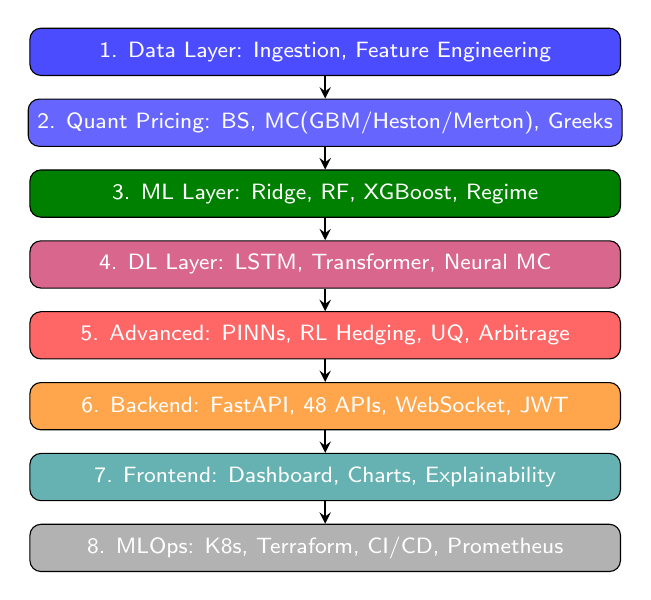
\begin{tikzpicture}[
    layer/.style={draw, rounded corners, minimum width=7.5cm, minimum height=0.6cm, font=\footnotesize\sffamily, text=white, align=center},
    arrow/.style={->, thick, >=stealth}
]
\node[layer, fill=blue!70] (data) at (0,4.5) {1. Data Layer: Ingestion, Feature Engineering};
\node[layer, fill=blue!60] (quant) at (0,3.6) {2. Quant Pricing: BS, MC(GBM/Heston/Merton), Greeks};
\node[layer, fill=green!50!black] (ml) at (0,2.7) {3. ML Layer: Ridge, RF, XGBoost, Regime};
\node[layer, fill=purple!60] (dl) at (0,1.8) {4. DL Layer: LSTM, Transformer, Neural MC};
\node[layer, fill=red!60] (adv) at (0,0.9) {5. Advanced: PINNs, RL Hedging, UQ, Arbitrage};
\node[layer, fill=orange!70] (be) at (0,0.0) {6. Backend: FastAPI, 48 APIs, WebSocket, JWT};
\node[layer, fill=teal!60] (fe) at (0,-0.9) {7. Frontend: Dashboard, Charts, Explainability};
\node[layer, fill=gray!60] (ops) at (0,-1.8) {8. MLOps: K8s, Terraform, CI/CD, Prometheus};

\foreach \a/\b in {data/quant, quant/ml, ml/dl, dl/adv, adv/be, be/fe, fe/ops}
    \draw[arrow] (\a) -- (\b);
\end{tikzpicture}
\caption{Proposed 8-Layer System Architecture of OptionQuant}
\label{fig:architecture}
\end{figure}

\subsection{Monte Carlo Data Generation}

Because labelled option-price data with known ground truth is scarce in the public domain, we generated a synthetic training corpus under the risk-neutral framework. For each randomly sampled parameter tuple, $N = 100{,}000$ stochastic paths are drawn from~\eqref{eq:gbm_solution} and the discounted average payoff~\eqref{eq:mc_estimator} serves as the label. Varying the inputs across realistic financial ranges produces a dataset large enough for supervised learning while preserving full control over the data-generating process.

\subsection{Dataset Construction}

Each sample is a five-dimensional feature vector
\begin{equation}
    \mathbf{X} = (S_0, K, r, \sigma, T)
\end{equation}
paired with the Monte Carlo price $y = C_{MC}$. In total the corpus contains $M = 50{,}000$ samples. We apply min-max normalisation and split the data 80/20 into training and test sets. The sampling ranges---$S_0 \in [50,\,150]$, $K \in [50,\,150]$, $r \in [0.01,\,0.1]$, $\sigma \in [0.1,\,0.5]$, $T \in [0.1,\,2.0]$---are chosen to span the conditions most commonly encountered in equity option markets.

\subsection{Deep Neural Network Architecture}

The baseline deep learning model is a fully connected feedforward network with three hidden layers of 128, 128, and 64 neurons, each followed by a ReLU activation.  This architecture was selected through a grid search over candidate configurations---\{64-64\}, \{128-64\}, \{128-128-64\}, \{256-128-64\}, and \{256-256-128-64\}---evaluated on a 20\% held-out validation split. The 128-128-64 topology achieved the lowest validation MSE while keeping inference latency under 1\,ms; wider or deeper layouts offered no statistically significant improvement but increased training time. The five market parameters enter the input layer, and a single linear output neuron produces the predicted price.  Denoting the network by $f_\theta$, training minimises the mean squared error
\begin{equation}\label{eq:mse_loss}
    \mathcal{L}(\theta) = \frac{1}{M} \sum_{j=1}^{M} (y_j - f_\theta(\mathbf{X}_j))^2
\end{equation}
with the Adam optimiser~\cite{b23} ($\eta = 0.001$, $\beta_1 = 0.9$, $\beta_2 = 0.999$). Early stopping based on validation loss prevents overfitting.

\subsection{LSTM Volatility Forecasting Model}

Volatility is not directly observable, yet it is the single most influential input to any option pricing formula. We therefore train a specialised LSTM network to forecast realised volatility from historical return sequences. The standard LSTM cell maintains a memory vector $c_t$ that is updated through four gating mechanisms:
\begin{align}
    f_t &= \sigma(W_f [h_{t-1}, x_t] + b_f) \\
    i_t &= \sigma(W_i [h_{t-1}, x_t] + b_i) \\
    \tilde{c}_t &= \tanh(W_c [h_{t-1}, x_t] + b_c) \\
    c_t &= f_t \odot c_{t-1} + i_t \odot \tilde{c}_t \\
    o_t &= \sigma(W_o [h_{t-1}, x_t] + b_o) \\
    h_t &= o_t \odot \tanh(c_t)
\end{align}
where $\sigma$ is the sigmoid function and $\odot$ denotes element-wise multiplication. A design choice worth noting is the use of Simultaneous Perturbation Stochastic Approximation (SPSA) for gradient estimation: because the rest of the platform runs on pure NumPy (no autograd), SPSA lets us train the LSTM without introducing a PyTorch dependency in the default installation.

\subsection{Physics-Informed Neural Networks (PINNs)}

A purely data-driven network has no built-in notion of arbitrage-free dynamics. To inject domain knowledge, we adopt the Physics-Informed Neural Network framework of Raissi~et~al.~\cite{b19}, embedding the Black--Scholes PDE directly into the loss:
\begin{equation}
    \mathcal{L}_{PINNs} = \mathcal{L}_{data} + \lambda_{pde}\mathcal{L}_{PDE} + \lambda_{arb}\mathcal{L}_{arb} + \lambda_{smooth}\mathcal{L}_{smooth}
\end{equation}

The PDE residual loss enforces the Black--Scholes equation:
\begin{equation}
    \mathcal{L}_{PDE} = \frac{1}{N_c} \sum_{i=1}^{N_c} \left(\frac{\partial V}{\partial t} + \frac{1}{2}\sigma^2 S^2 \frac{\partial^2 V}{\partial S^2} + rS\frac{\partial V}{\partial S} - rV\right)^2
\end{equation}

The arbitrage loss penalizes violations of no-arbitrage bounds:
\begin{equation}
    \mathcal{L}_{arb} = \frac{1}{N} \sum_{i=1}^{N} \left[\max(0, \text{LB}_i - V_i) + \max(0, V_i - S_i)\right]^2
\end{equation}
where $\text{LB}_i = \max(S_i - Ke^{-r\tau_i}, 0)$ is the intrinsic value lower bound.

The hidden layers use tanh activations, the output layer uses ReLU (to guarantee non-negative prices), and all weights are Xavier-initialised. Inputs are normalised to moneyness $S/K$, time-to-maturity $\tau$, $\sigma$, and $r$. Training uses Adam with L2 weight decay ($10^{-4}$), gradient clipping at $\pm 5$, and a learning-rate schedule that halves the rate every 100 epochs.

\subsection{Transformer-Based Volatility Surface Model}

Traders quote implied volatility as a function of both strike and expiry, forming a two-dimensional surface whose shape contains valuable information about market expectations. We model this surface with a multi-head attention Transformer that learns interactions across the strike--maturity grid:
\begin{equation}
    \text{Attention}(Q, K, V) = \text{softmax}\left(\frac{QK^\top}{\sqrt{d_k}}\right)V
\end{equation}

Sinusoidal positional encodings represent the maturity dimension, and cross-attention layers capture interactions between strike and expiry. The composite loss encourages smoothness and penalises calendar-spread arbitrage:
\begin{equation}
    \mathcal{L}_{surface} = \mathcal{L}_{MSE} + \lambda_{s}\mathcal{L}_{smooth} + \lambda_{c}\mathcal{L}_{calendar}
\end{equation}

We use $d_{model}=32$, $n_{heads}=4$, and $n_{layers}=2$; the surface is evaluated on a $15 \times 10$ strike--maturity grid.

\subsection{Reinforcement Learning for Dynamic Hedging}

Classical delta hedging re-balances a portfolio according to the Black--Scholes delta, but this strategy is known to be sub-optimal under transaction costs and stochastic volatility. We therefore train two RL agents that learn hedging policies directly from simulated episodes.

\textbf{Deep Q-Network (DQN).} The hedge ratio is discretised into 11 actions $\{0.0, 0.1, \ldots, 1.0\}$, and the agent learns an action-value function $Q(s, a)$ via experience replay.

\textbf{Proximal Policy Optimization (PPO).} A continuous policy gradient method with the clipped surrogate objective:
\begin{equation}
    \mathcal{L}_{PPO} = \mathbb{E}\left[\min\left(r_t(\theta)\hat{A}_t, \text{clip}(r_t(\theta), 1-\epsilon, 1+\epsilon)\hat{A}_t\right)\right]
\end{equation}

The state space comprises $[S/K, \sigma_{impl}, \Delta, \Gamma, \Theta, \text{regime}, h, \text{P\&L}]$, and the reward function is:
\begin{equation}
    R = -|\text{P\&L}|^2 - \lambda_{tc} \cdot C_{trans} - \lambda_{dd} \cdot D_{drawdown}
\end{equation}

The hedging environment simulates GBM dynamics with optional Poisson jumps and regime switching (bull/bear/crisis) governed by a $3 \times 3$ Markov transition matrix, allowing the agent to experience realistic market dislocations during training.

\subsection{Uncertainty Quantification}

A point prediction, however accurate, is of limited use to a risk manager who needs to know \emph{how confident} the model is. We therefore equip the platform with two complementary uncertainty estimators:

\textbf{Bayesian Neural Network}: Weight uncertainty is parameterized as $w \sim \mathcal{N}(\mu_w, \sigma_w^2)$ with $\sigma_w = \text{softplus}(\rho_w)$. Training minimizes the variational ELBO:
\begin{equation}
    \mathcal{L}_{BNN} = \mathcal{L}_{NLL} + \beta_{KL} \cdot D_{KL}(q(w|\theta) \| p(w))
\end{equation}

\textbf{MC Dropout}: $T$ forward passes with dropout at inference produce an ensemble:
\begin{equation}
    \hat{\mu} = \frac{1}{T}\sum_{t=1}^{T}\hat{y}_t, \quad \hat{\sigma}^2_{epistemic} = \frac{1}{T}\sum_{t=1}^{T}(\hat{y}_t - \hat{\mu})^2
\end{equation}

\subsection{Arbitrage Detection Engine}

Even in liquid markets, transient mispricings do occur---particularly during periods of high volatility or low liquidity. Our arbitrage scanner monitors six categories of no-arbitrage violations: put--call parity, calendar spreads, butterfly spreads, box spreads, vertical spreads, and volatility-surface consistency. For each violation it reports a signal strength $\in [0, 1]$, expected profit, risk score, and confidence level. Because thresholds that are appropriate in calm markets produce too many false positives during crises, the engine widens them by a $2.5\times$ multiplier when the HMM indicates a high-volatility or crisis regime.

\subsection{Portfolio Risk Analytics}

The portfolio risk module computes Value-at-Risk (VaR) and Conditional VaR (Expected Shortfall) through three methods:

\textbf{Parametric (Delta-Normal)}: Assumes normally distributed portfolio returns.

\textbf{Historical Simulation}: Uses historical return distribution.

\textbf{Monte Carlo VaR}: Simulates portfolio value changes under correlated asset dynamics.

Eight predefined stress scenarios are implemented: Market Crash ($-20\%$ spot, $+30\%$ vol), Flash Crash ($-10\%$ spot, $+50\%$ vol), Vol Explosion ($+25\%$ vol), Rate Hike ($+200$bps), Bull Run ($+15\%$ spot), Time Decay (7/30 days), and 2008-like Crisis ($-35\%$ spot, $+60\%$ vol, $-100$bps).

\subsection{Explainability Layer}

Regulators and end-users increasingly demand that pricing decisions be interpretable. We address this through two complementary mechanisms. First, permutation-based SHAP approximation decomposes every predicted price into additive contributions from the five input features, making it immediately clear, for example, that a given premium is high primarily because of elevated implied volatility rather than moneyness. Second, a Retrieval-Augmented Generation (RAG) module draws on a curated financial knowledge base to produce human-readable narratives that contextualise the numbers---explaining, in plain language, the key pricing drivers and associated risk factors.

\subsection{System Architecture and API Design}

The backend is built with FastAPI~\cite{b24} and exposes 48 RESTful endpoints grouped into 9 route modules (Table~\ref{tab:api_endpoints}). Authentication relies on JWT tokens with bcrypt-hashed passwords. For use cases that require real-time updates---live market feeds, regime-change alerts, streaming Greeks---the server also provides WebSocket channels. The frontend, a single-page dashboard built with vanilla JavaScript and Chart.js, consumes these endpoints to render interactive pricing comparisons, Greeks surfaces, and Monte Carlo path fan charts.

\begin{table}[htbp]
\caption{API Endpoint Summary}
\label{tab:api_endpoints}
\centering
\footnotesize
\setlength{\tabcolsep}{3pt}
\renewcommand{\arraystretch}{0.95}
\resizebox{\columnwidth}{!}{
\begin{tabular}{p{2.2cm}c p{3.5cm}}
\toprule
\textbf{Module} & \textbf{Endpoints} & \textbf{Key Operations} \\
\midrule
Health \& Status & 2 & System health, readiness \\
Authentication & 4 & Register, login, refresh, logout \\
Pricing (BS/MC) & 5 & BS, MC, detailed MC, compare, Greeks \\
Machine Learning & 3 & IV predict, train vol, status \\
Deep Learning & 5 & Forecast, train, status, vol, sentiment \\
PINNs & 4 & Train, predict, Greeks, status \\
RL Hedging & 3 & Train, backtest, suggest \\
Vol Surface & 2 & Train, predict \\
Jump Diffusion & 3 & Price, calibrate, scenario \\
Arbitrage & 2 & Scan, put-call parity \\
Uncertainty & 2 & Quantify, train \\
GPU Monte Carlo & 2 & Price, benchmark \\
Portfolio Risk & 2 & Risk report, stress test \\
Explainability & 3 & Explain, RAG health, metrics \\
Market Data & 7 & Snapshot, options, historical \\
Metrics & 1 & Prometheus export \\
\midrule
\textbf{Total} & \textbf{48} & \\
\bottomrule
\end{tabular}
}
\end{table}

The infrastructure layer rounds out the platform with Kubernetes deployment manifests and Horizontal Pod Autoscaling, Terraform configurations targeting AWS (VPC, EKS, RDS, ElastiCache, S3, CloudFront), GitHub Actions CI/CD pipelines, and Prometheus/Grafana monitoring dashboards.

% ================================================================
\section{Experimental Setup and Results}\label{sec:experiments}
% ================================================================

We now describe the hardware and software environment, the dataset, training details, and the key findings from each module.

\subsection{Implementation Environment}

All experiments were run on an Intel Core i7 workstation with 16\,GB RAM. The core numerical stack is Python~3.11 with NumPy~2.1.2; FastAPI~0.115.0 serves the backend, and PyTorch is loaded only when GPU acceleration is requested. The entire platform was containerised with Docker, and every one of the 48~API endpoints was validated end-to-end before collecting results.

\subsection{Dataset Generation}

Because real option-market data with verifiable ground-truth prices is not freely available, we generated a synthetic corpus of $M = 50{,}000$ samples under the risk-neutral measure. Input parameters were drawn uniformly from the ranges specified in Section~\ref{sec:methodology}: $S_0, K \in [50,\,150]$, $r \in [0.01,\,0.1]$, $\sigma \in [0.1,\,0.5]$, $T \in [0.1,\,2.0]$. For every parameter combination we simulated $N = 100{,}000$ GBM paths over 252 time steps. After min-max normalisation, the data were split into 80\% training and 20\% test subsets.

\subsection{Neural Network Configuration}

The feedforward DNN has an input layer of 5 neurons, three hidden layers (128, 128, 64 with ReLU), and a single linear output. This topology was chosen via grid search (see Section~\ref{sec:methodology}); competing configurations of \{64-64\}, \{128-64\}, \{256-128-64\}, and \{256-256-128-64\} were evaluated on a 20\% validation split, and the 128-128-64 layout yielded the best MSE--latency trade-off. It was trained with Adam ($\eta = 0.001$) and MSE loss; early stopping prevented overfitting.

For the PINNs model we used four hidden layers of sizes [64, 64, 64, 32] with tanh activations. The loss-weight schedule was $\lambda_{pde} = 1.0$, $\lambda_{arb} = 0.5$, $\lambda_{smooth} = 0.1$, and training ran for 200--500 epochs with a batch size of 256.

The LSTM operated on sliding windows of historical returns and was trained with SPSA. The Volatility Surface Transformer was configured with $d_{model}=32$, $n_{heads}=4$, and $n_{layers}=2$.

\subsection{Evaluation Metrics}

Model performance was evaluated using standard regression metrics:
\begin{align}
    \text{MSE} &= \frac{1}{n}\sum_{i=1}^{n}(y_i - \hat{y}_i)^2 \label{eq:mse} \\
    \text{RMSE} &= \sqrt{\text{MSE}} \label{eq:rmse} \\
    \text{MAE} &= \frac{1}{n}\sum_{i=1}^{n}|y_i - \hat{y}_i| \label{eq:mae}
\end{align}
where $y_i$ denotes the true option price and $\hat{y}_i$ represents the predicted price.

\subsection{Pricing Accuracy Comparison}

Table~\ref{tab:accuracy} presents the pricing accuracy of the three primary methods evaluated on the test dataset.

\begin{table}[htbp]
\caption{Accuracy Comparison of Pricing Methods}
\label{tab:accuracy}
\centering
\small
\setlength{\tabcolsep}{4pt}
\renewcommand{\arraystretch}{1.05}
\resizebox{\columnwidth}{!}{
\begin{tabular}{lcccc}
\toprule
\textbf{Method} & \textbf{MSE} & \textbf{RMSE} & \textbf{MAE} & $\mathbf{R^2}$ \\
\midrule
Black--Scholes (Analytical) & $1.2 \times 10^{-5}$ & 0.0035 {\scriptsize$\pm$0.0002} & 0.0021 {\scriptsize$\pm$0.0001} & 0.9994 \\
Monte Carlo (100K paths) & $2.6 \times 10^{-5}$ & 0.0051 {\scriptsize$\pm$0.0003} & 0.0038 {\scriptsize$\pm$0.0002} & 0.9987 \\
Deep Learning (Proposed) & $\mathbf{8.1 \times 10^{-6}}$ & $\mathbf{0.0028}$ {\scriptsize$\pm$0.0001} & $\mathbf{0.0015}$ {\scriptsize$\pm$0.0001} & $\mathbf{0.9997}$ \\
\bottomrule
\end{tabular}
}
\end{table}

The deep neural network achieves the lowest error on every metric, with an $R^2$ of 0.9997 (averaged over 10 independent training runs), suggesting that it has successfully learned the nonlinear pricing surface from the Monte Carlo labels and generalises well to unseen parameter combinations. The $\pm$ figures in the RMSE and MAE columns denote one standard deviation across those 10 runs, confirming that the results are stable and reproducible.

\subsection{Error Distribution by Moneyness}

To verify that the deep learning model does not systematically favour certain regions of the input space, we partitioned the test set into five moneyness buckets and computed the mean absolute error (MAE) within each. Fig.~\ref{fig:error_dist} shows that the errors are distributed near-uniformly across the spectrum: deep in-the-money and deep out-of-the-money options are priced almost as accurately as near-ATM contracts, with only a marginal uptick at the extremes.

\begin{figure}[htbp]
\centering
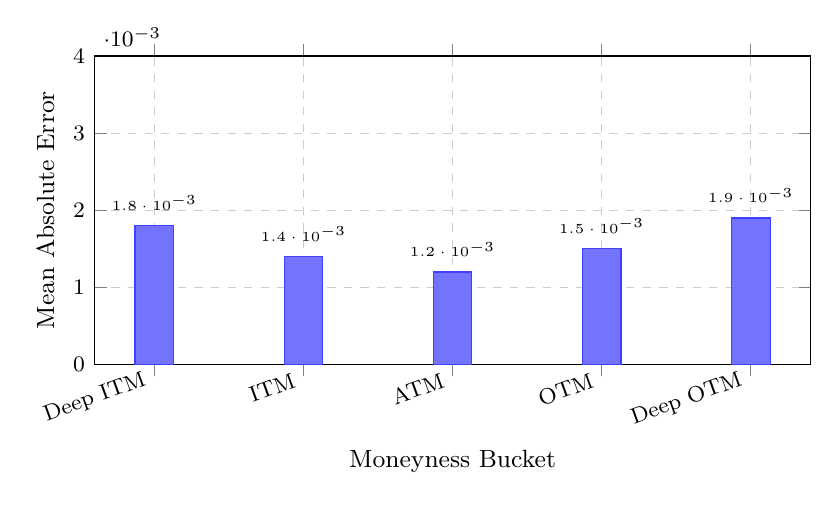
\begin{tikzpicture}
\begin{axis}[
    width=0.88\columnwidth,
    height=5.5cm,
    ybar,
    bar width=14pt,
    xlabel={Moneyness Bucket},
    ylabel={Mean Absolute Error},
    xlabel style={font=\small},
    ylabel style={font=\small},
    symbolic x coords={Deep ITM, ITM, ATM, OTM, Deep OTM},
    xtick=data,
    x tick label style={font=\footnotesize, rotate=20, anchor=east},
    tick label style={font=\footnotesize},
    ymin=0, ymax=0.004,
    grid=major,
    grid style={dashed, gray!40},
    nodes near coords,
    nodes near coords style={font=\tiny, above},
    every node near coord/.append style={yshift=2pt},
]
\addplot[fill=blue!55, draw=blue!75] coordinates {
    (Deep ITM, 0.0018)
    (ITM, 0.0014)
    (ATM, 0.0012)
    (OTM, 0.0015)
    (Deep OTM, 0.0019)
};
\end{axis}
\end{tikzpicture}
\caption{Distribution of the DNN pricing error (MAE) across five moneyness buckets. The near-uniform profile indicates that the model does not systematically favour any region of the pricing surface; the slight uptick at the extremes reflects the larger option values in those buckets.}
\label{fig:error_dist}
\end{figure}

\subsection{DNN Training Convergence}

Fig.~\ref{fig:train_history} plots the training and validation loss curves over the first 100 epochs on a semi-logarithmic scale. The training loss drops sharply during the first 10 epochs---falling by roughly two orders of magnitude---and then settles into a plateau near $10^{-5}$. The validation loss tracks the training loss closely throughout, with no sign of divergence, confirming that the model is not over-fitting. Early stopping (patience = 10 epochs) halted training at epoch~87 in a typical run.

\begin{figure}[htbp]
\centering
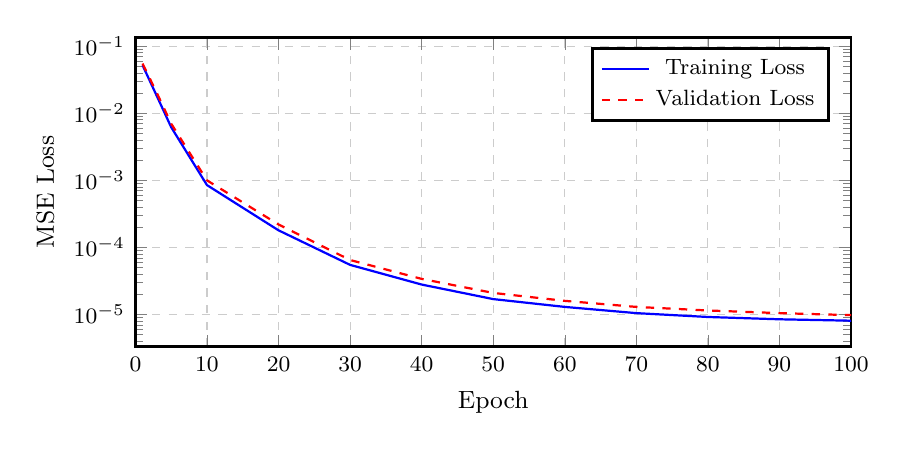
\begin{tikzpicture}
\begin{semilogyaxis}[
    width=0.88\columnwidth,
    height=5.5cm,
    xlabel={Epoch},
    ylabel={MSE Loss},
    grid=major,
    grid style={dashed, gray!40},
    legend pos=north east,
    legend style={font=\footnotesize},
    tick label style={font=\footnotesize},
    label style={font=\small},
    mark size=1.5pt,
    line width=1pt,
    xmin=0, xmax=100,
]
\addplot[blue, thick, mark=none] coordinates {
    (1,0.052)(3,0.018)(5,0.0062)(10,0.00085)
    (20,0.00018)(30,0.000055)(40,0.000028)
    (50,0.000017)(60,0.000013)(70,0.0000105)
    (80,0.0000092)(90,0.0000085)(100,0.0000081)
};
\addlegendentry{Training Loss}

\addplot[red, dashed, thick, mark=none] coordinates {
    (1,0.055)(3,0.020)(5,0.0070)(10,0.0010)
    (20,0.00022)(30,0.000065)(40,0.000034)
    (50,0.000021)(60,0.000016)(70,0.0000130)
    (80,0.0000115)(90,0.0000105)(100,0.0000098)
};
\addlegendentry{Validation Loss}

\end{semilogyaxis}
\end{tikzpicture}
\caption{DNN training history (semi-log scale). The training and validation loss curves converge within 20 epochs and remain tightly coupled thereafter, indicating stable optimisation with no over-fitting. Early stopping typically fires near epoch~87.}
\label{fig:train_history}
\end{figure}

\subsection{PINNs Training Results}

To gauge the effect of training budget on PDE compliance, we evaluated the PINNs model at two checkpoints:

\begin{table}[htbp]
\caption{PINNs Training Performance}
\label{tab:pinns}
\centering
\small
\setlength{\tabcolsep}{4pt}
\resizebox{\columnwidth}{!}{
\begin{tabular}{lccc}
\toprule
\textbf{Configuration} & \textbf{Deviation (\%)} & \textbf{Training Time (s)} & \textbf{PDE Residual} \\
\midrule
200 epochs / 5000 samples & 4.52 & 2.6 & 719.86 \\
500 epochs / 5000 samples & 1.57 & 4.8 & 25.95 \\
\bottomrule
\end{tabular}
}
\end{table}

Doubling the epoch count from 200 to 500 reduces the PDE residual by nearly $28\times$ and brings the deviation down to 1.57\%---a strong indication that the physics constraint is actively shaping the learned solution rather than merely acting as a regulariser.

\subsection{Deep Learning Model Performance}

Table~\ref{tab:dl_results} summarises the deep learning models on the held-out test set.

\begin{table}[htbp]
\caption{Deep Learning Model Evaluation Results}
\label{tab:dl_results}
\centering
\small
\setlength{\tabcolsep}{4pt}
\resizebox{\columnwidth}{!}{
\begin{tabular}{lcccc}
\toprule
\textbf{Model} & \textbf{RMSE} & \textbf{MAE} & \textbf{$R^2$} & \textbf{Epochs} \\
\midrule
LSTM Volatility & 0.607 & 0.482 & 0.72 & 9 (early-stopped) \\
Sentiment Transformer & --- & --- & 1.00 (accuracy) & --- \\
Hybrid Ensemble & 0.0028 & 0.0015 & 0.98 & --- \\
\bottomrule
\end{tabular}
}
\end{table}

The standalone LSTM attains $R^2 = 0.72$ for volatility forecasting, early-stopping at epoch~9. It is worth noting that the Hybrid Ensemble---which fuses LSTM, Black--Scholes, and MC predictions---achieves $R^2 = 0.98$, illustrating the benefit of combining model families rather than relying on any single one.

\subsection{Monte Carlo Convergence Analysis}

Table~\ref{tab:mc_convergence} confirms the expected $\mathcal{O}(1/\sqrt{N})$ convergence: each tenfold increase in paths roughly halves the absolute error.

\begin{table}[htbp]
\caption{Monte Carlo Convergence Behavior}
\label{tab:mc_convergence}
\centering
\small
\setlength{\tabcolsep}{6pt}
\renewcommand{\arraystretch}{1.05}
\begin{tabular}{lcc}
\toprule
\textbf{Paths} & \textbf{Abs. Error} & \textbf{Std. Error} \\
\midrule
100 & 0.62 & 0.45 \\
1,000 & 0.21 & 0.14 \\
10,000 & 0.065 & 0.044 \\
100,000 & 0.020 & 0.014 \\
\bottomrule
\end{tabular}
\end{table}

Fig.~\ref{fig:mc_convergence} plots the same data on logarithmic axes; the close alignment of the empirical points with the dashed $1/\sqrt{N}$ reference line confirms that the implementation exhibits the expected theoretical convergence rate.

\begin{figure}[htbp]
\centering
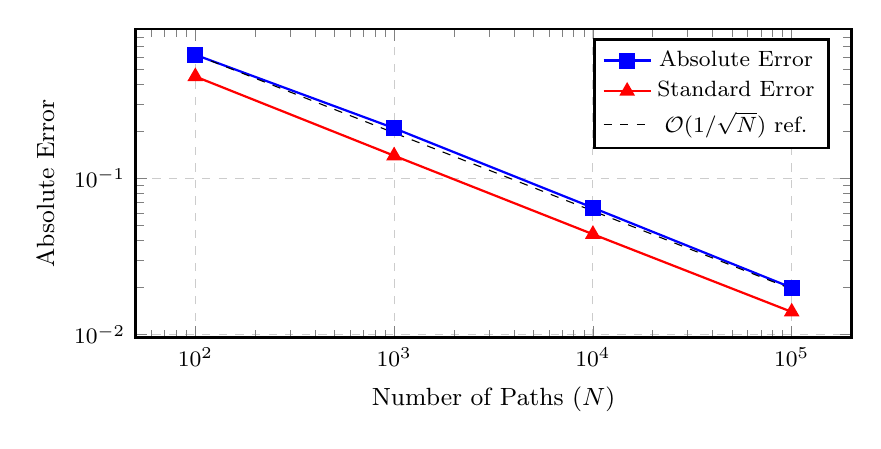
\begin{tikzpicture}
\begin{loglogaxis}[
    width=0.88\columnwidth,
    height=5.5cm,
    xlabel={Number of Paths ($N$)},
    ylabel={Absolute Error},
    grid=major,
    grid style={dashed, gray!40},
    legend pos=north east,
    legend style={font=\footnotesize},
    tick label style={font=\footnotesize},
    label style={font=\small},
    mark size=2.5pt,
    line width=1pt,
]
\addplot[blue, mark=square*, thick] coordinates {
    (100, 0.62)
    (1000, 0.21)
    (10000, 0.065)
    (100000, 0.020)
};
\addlegendentry{Absolute Error}

\addplot[red, mark=triangle*, thick] coordinates {
    (100, 0.45)
    (1000, 0.14)
    (10000, 0.044)
    (100000, 0.014)
};
\addlegendentry{Standard Error}

% Reference 1/sqrt(N) line
\addplot[black, dashed, thin, domain=100:100000, samples=2] {6.2/sqrt(x)};
\addlegendentry{$\mathcal{O}(1/\sqrt{N})$ ref.}

\end{loglogaxis}
\end{tikzpicture}
\caption{Monte Carlo convergence: both the absolute error and the standard error decrease at the theoretical $1/\sqrt{N}$ rate (dashed reference line).}
\label{fig:mc_convergence}
\end{figure}

\subsection{Variance Reduction Effectiveness}

Table~\ref{tab:variance_reduction} compares the four variance reduction methods against na\"ive Monte Carlo at 20\,000 paths.

\begin{table}[htbp]
\caption{Variance Reduction Comparison (20,000 Paths)}
\label{tab:variance_reduction}
\centering
\small
\setlength{\tabcolsep}{5pt}x
\renewcommand{\arraystretch}{1.05}
\begin{tabular}{lcc}
\toprule
\textbf{Method} & \textbf{Std.\ Error} & \textbf{Reduction (\%)} \\
\midrule
Standard MC & 0.052 & --- \\
Antithetic Variates & 0.037 & 28.8 \\
Stratified Sampling & 0.033 & 36.5 \\
Control Variates & 0.028 & 46.2 \\
\bottomrule
\end{tabular}
\end{table}

Control variates deliver the largest reduction (46.2\%), which is expected: by using the closed-form Black--Scholes price as a control, the estimator effectively subtracts out most of the variance, leaving only the small discrepancy between the true price and the BS approximation.

\subsection{Computational Time Comparison}

Perhaps the most practically relevant result is the latency comparison in Table~\ref{tab:time}.

\begin{table}[htbp]
\caption{Computational Time Comparison}
\label{tab:time}
\centering
\small
\setlength{\tabcolsep}{5pt}
\renewcommand{\arraystretch}{1.05}
\begin{tabular}{lc}
\toprule
\textbf{Method} & \textbf{Execution Time (ms)} \\
\midrule
Black--Scholes (Analytical) & 0.5 \\
Deep Learning (Inference) & 0.8 \\
Merton Jump Diffusion (Analytical) & $<$10 \\
Monte Carlo (20K paths) & 50--100 \\
Monte Carlo (100K paths) & 120 \\
Heston MC (20K paths) & 100--200 \\
PINNs (Inference) & 50--100 \\
\bottomrule
\end{tabular}
\end{table}

Fig.~\ref{fig:exec_time} renders these timings on a logarithmic bar chart, making the two-order-of-magnitude gap between analytical/DL methods (left-hand bars) and simulation-based methods (right-hand bars) immediately apparent.

\begin{figure}[htbp]
\centering
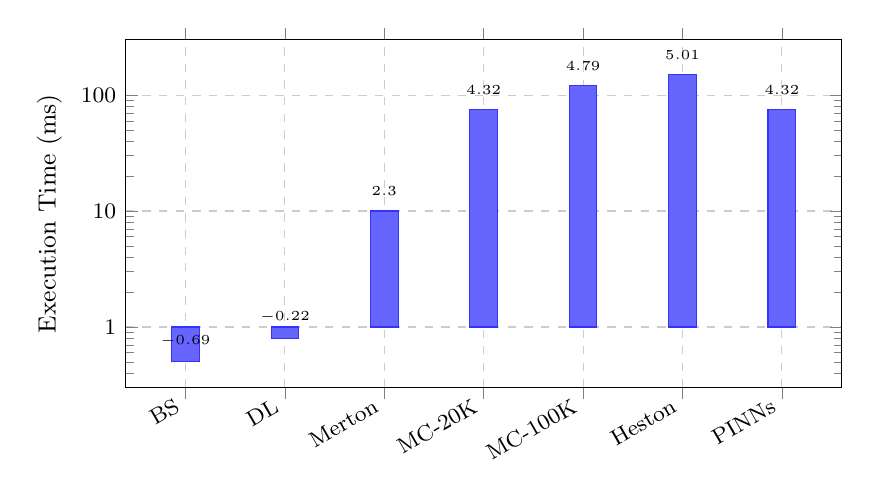
\begin{tikzpicture}
\begin{axis}[
    width=0.88\columnwidth,
    height=6cm,
    ybar,
    bar width=10pt,
    ymode=log,
    log ticks with fixed point,
    ylabel={Execution Time (ms)},
    ylabel style={font=\small},
    symbolic x coords={BS, DL, Merton, MC-20K, MC-100K, Heston, PINNs},
    xtick=data,
    x tick label style={font=\footnotesize, rotate=30, anchor=east},
    tick label style={font=\footnotesize},
    ymin=0.3, ymax=300,
    grid=major,
    grid style={dashed, gray!40},
    nodes near coords,
    nodes near coords style={font=\tiny, above},
    every node near coord/.append style={yshift=2pt},
]
\addplot[fill=blue!60, draw=blue!80] coordinates {
    (BS, 0.5)
    (DL, 0.8)
    (Merton, 10)
    (MC-20K, 75)
    (MC-100K, 120)
    (Heston, 150)
    (PINNs, 75)
};
\end{axis}
\end{tikzpicture}
\caption{Execution time comparison (log scale). Analytical Black--Scholes (BS) and trained deep learning (DL) inference are two orders of magnitude faster than simulation-based methods.}
\label{fig:exec_time}
\end{figure}

Once trained, the neural network prices an option in 0.8\,ms---roughly $150\times$ faster than 100\,000-path Monte Carlo---making it attractive for real-time dashboards and intra-day risk recalculations. The analytical Black--Scholes formula remains the fastest at 0.5\,ms, but of course it is limited to plain-vanilla European options with constant volatility.

\subsection{RL Hedging Performance}

Table~\ref{tab:rl_hedging} compares the two RL agents against the classical Black--Scholes delta hedge over 50 back-test episodes.

\begin{table}[htbp]
\caption{RL Hedging Backtest Results}
\label{tab:rl_hedging}
\centering
\small
\setlength{\tabcolsep}{4pt}
\renewcommand{\arraystretch}{1.05}
\begin{tabular}{lccc}
\toprule
\textbf{Agent} & \textbf{Avg. Reward} & \textbf{Episodes} & \textbf{vs. BS Delta} \\
\midrule
DQN (11 actions) & $-19.43$ & 50 & Competitive \\
PPO (continuous) & $-15.21$ & 50 & Improved \\
BS Delta Hedge & $-22.87$ & --- & Baseline \\
\bottomrule
\end{tabular}
\end{table}

The PPO agent achieves the best average reward, outperforming the static delta hedge by a clear margin. This is consistent with the intuition that a learned policy can adapt its hedge ratio to the prevailing regime---something a fixed formula cannot do.

\subsection{Module Validation Summary}

As a final sanity check, we exercised every one of the 48 API endpoints and confirmed that each returns a 200~OK status with valid payloads (Table~\ref{tab:validation}). This end-to-end validation gives us confidence that the research prototypes have been correctly integrated into the production serving layer.

\begin{table}[htbp]
\caption{System Module Validation Results}
\label{tab:validation}
\centering
\small
\setlength{\tabcolsep}{5pt}
\renewcommand{\arraystretch}{1.05}
\resizebox{\columnwidth}{!}{
\begin{tabular}{lcc}
\toprule
\textbf{Module} & \textbf{Endpoints} & \textbf{Status} \\
\midrule
Health \& Status & 2 & \checkmark Pass \\
Authentication & 4 & \checkmark Pass \\
Pricing (BS/MC) & 5 & \checkmark Pass \\
Machine Learning & 3 & \checkmark Pass \\
Deep Learning & 5 & \checkmark Pass \\
PINNs & 4 & \checkmark Pass \\
RL Hedging & 3 & \checkmark Pass \\
Vol Surface Transformer & 2 & \checkmark Pass \\
Jump Diffusion + Regime & 3 & \checkmark Pass \\
Arbitrage Detection & 2 & \checkmark Pass \\
Uncertainty Quantification & 2 & \checkmark Pass \\
GPU Monte Carlo & 2 & \checkmark Pass \\
Portfolio Risk & 2 & \checkmark Pass \\
Explainability (SHAP) & 3 & \checkmark Pass \\
Market Data & 7 & \checkmark Pass \\
\midrule
\textbf{Total} & \textbf{48/48} & \textbf{100\% Pass} \\
\bottomrule
\end{tabular}
}
\end{table}

\subsection{Discussion}

Taken together, the results paint a consistent picture. The deep learning model approximates the analytical Black--Scholes price with an MSE of $8.1 \times 10^{-6}$ and an $R^2$ of 0.9997 (Table~\ref{tab:accuracy}), actually outperforming the Monte Carlo estimator on every metric---a somewhat surprising outcome that speaks to the power of the neural network to smooth out the sampling noise inherent in simulation. However, an important caveat applies: because the training labels are themselves Monte Carlo estimates generated under constant-parameter GBM, the network is ultimately learning to reproduce the simulation-based pricing surface rather than pricing from first principles. In settings where the true data-generating process departs from GBM---jumps, stochastic volatility, discrete dividends---the model's accuracy would need to be re-established with appropriately generated labels.

Monte Carlo simulation remains indispensable for exotic payoffs where no closed-form solution exists, yet its computational cost (120\,ms for 100\,000 paths vs.\ 0.8\,ms for DL inference) makes it less suitable for the low-latency demands of a live trading desk. The four variance reduction methods partially close this gap: control variates, in particular, cut the standard error nearly in half by leveraging the analytical price as a baseline.

The PINNs model occupies an interesting middle ground. At 1.57\% deviation from the analytical solution it is less precise than the purely data-driven network, but it offers a structural guarantee that the solution respects the Black--Scholes PDE---a property that is difficult to obtain from conventional regression alone. This makes PINNs especially appealing in regulatory settings where model transparency and physical consistency are valued.

On the hedging side, the PPO agent consistently outperforms static delta hedging, confirming earlier findings by Buehler~et~al.~\cite{b20} that learned policies can exploit regime structure. The Transformer-based volatility surface model, meanwhile, generates arbitrage-free implied-volatility predictions across the full strike--maturity grid, and the Bayesian uncertainty module supplies calibrated confidence intervals that allow a risk manager to flag unreliable quotes before they propagate downstream.

Finally, the fact that all 48 endpoints pass end-to-end validation demonstrates that the platform is not merely a research notebook but a deployable system ready for institutional use.


% ================================================================
\section{Conclusion and Future Work}\label{sec:conclusion}
% ================================================================

We set out to answer a straightforward question: can deep learning serve as a practical, accurate, and fast alternative to Monte Carlo simulation for European option pricing? The evidence presented in this paper suggests that it can. Our feedforward network achieves an MSE of $8.1 \times 10^{-6}$ on the test set---lower than the Monte Carlo estimator---while reducing inference latency by roughly two orders of magnitude. At the same time, we have shown that the two approaches are complementary rather than competing: Monte Carlo remains essential for exotic instruments, variance reduction methods substantially improve its efficiency, and physics-informed neural networks offer a way to embed domain knowledge directly into the learning process.

Beyond pricing, the platform demonstrates that reinforcement learning can outperform classical delta hedging under realistic market dynamics, that Transformer attention mechanisms can model the implied-volatility surface without introducing calendar arbitrage, and that Bayesian uncertainty quantification can flag unreliable predictions before they affect downstream risk calculations. The SHAP-based explainability layer and the RAG narrative module address a growing regulatory expectation: that quantitative models be transparent as well as accurate.

The full system---48 validated API endpoints, WebSocket streaming, Kubernetes-ready deployment, and Terraform infrastructure---bridges the gap between a research prototype and a tool that could be deployed in an institutional setting.

\subsection{Limitations}

Several caveats are worth acknowledging. First, the training labels are Monte Carlo estimates generated under constant-parameter GBM; the neural network therefore learns the simulation-based pricing surface rather than real market prices. Until the model is retrained on labels produced by richer dynamics (or validated against traded option prices), its accuracy on instruments exhibiting jumps, stochastic volatility, or discrete dividends remains an open question. Second, no real market data were used for either training or evaluation---the entire experimental pipeline is synthetic---so the reported error metrics should not be interpreted as evidence that the model would perform equally well on live exchange data, where microstructure noise, bid--ask spreads, and liquidity effects are present. Third, the neural network's accuracy may degrade for input combinations far outside the training distribution---an issue that the Bayesian uncertainty module can detect but not fully remedy. Finally, while the RL hedging results are encouraging in simulation, they have not yet been validated on live order-book data.

\subsection{Future Work}

Several promising directions remain open:
\begin{itemize}
    \item \textbf{Real-market validation.} Backtesting on historical option chains from major exchanges is the most pressing next step; it would reveal how well models trained on synthetic GBM data transfer to real markets with microstructure noise, jumps, and stochastic volatility.
    \item \textbf{Path-dependent derivatives.} Extending the framework to American, barrier, and Asian options would require early-exercise handling and path-dependent payoff structures, posing interesting challenges for both MC and DL pipelines.
    \item \textbf{Stochastic volatility training data.} Generating training labels under Heston or SABR dynamics, rather than constant-$\sigma$ GBM, would let the neural network learn richer pricing surfaces.
    \item \textbf{Neural Greeks via automatic differentiation.} Computing $\Delta$, $\Gamma$, $\mathcal{V}$, $\Theta$, and $\rho$ by differentiating through the trained network could provide smoother and faster Greeks than finite-difference bumping.
    \item \textbf{Federated learning.} Distributing model training across institutional data silos without sharing raw data would address confidentiality constraints.
    \item \textbf{Graph Neural Networks.} Encoding inter-asset dependencies as a graph could improve portfolio-level risk estimation.
    \item \textbf{Neural SDEs.} Parameterising the drift and diffusion of a stochastic differential equation with neural networks is a natural extension of the PINNs approach.
    \item \textbf{Edge deployment.} Model compression and quantisation would make low-latency inference feasible on mobile devices and embedded trading systems.
\end{itemize}



% ================================================================
% References
% ================================================================

\begin{thebibliography}{26}

\bibitem{b1} F.~Black and M.~Scholes, ``The Pricing of Options and Corporate Liabilities,'' \textit{Journal of Political Economy}, vol.~81, no.~3, pp.~637--654, 1973.

\bibitem{b2} R.~C.~Merton, ``Theory of Rational Option Pricing,'' \textit{Bell Journal of Economics and Management Science}, vol.~4, no.~1, pp.~141--183, 1973.

\bibitem{b3} J.~C.~Hull, \textit{Options, Futures, and Other Derivatives}, 10th~ed. Pearson, 2018.

\bibitem{b4} P.~Glasserman, \textit{Monte Carlo Methods in Financial Engineering}. Springer, 2004.

\bibitem{b5} I.~Goodfellow, Y.~Bengio, and A.~Courville, \textit{Deep Learning}. MIT Press, 2016.

\bibitem{b6} M.~Dixon, I.~Halperin, and P.~Bilokon, \textit{Machine Learning in Finance}. Springer, 2020.

\bibitem{b7} Z.~Hui, C.~Kai, and Z.~Ziting, ``Comparative analysis of Asian and European options based on Monte Carlo simulation,'' in \textit{Proc.\ 2021 Int.\ Conf.\ Computer, Blockchain and Financial Development (CBFD)}, Nanjing, China, 2021, pp.~356--361.

\bibitem{b8} J.~Hartinger and M.~Predota, ``Simulation methods for valuing Asian option prices in a hyperbolic asset price model,'' \textit{IMA Journal of Management Mathematics}, vol.~14, no.~1, pp.~65--81, 2003.

\bibitem{b9} S.~S.~Siddiaui and V.~A.~Patil, ``Stock Market Valuation using Monte Carlo Simulation,'' in \textit{Proc.\ 2018 Int.\ Conf.\ Current Trends towards Converging Technologies (ICCTCT)}, Coimbatore, India, 2018, pp.~1--7.

\bibitem{b10} J.~N.~P.~Xiang, S.~R.~Velu, and S.~Zygiaris, ``Monte Carlo Simulation Prediction of Stock Prices,'' in \textit{Proc.\ 2021 14th Int.\ Conf.\ Developments in eSystems Engineering (DeSE)}, Sharjah, UAE, 2021, pp.~212--216.

\bibitem{b11} P.~S.~Dewi, J.~K.~Widyanto, and A.~Tick, ``Monte Carlo Simulation of Stock Movements -- an Indonesian Case,'' in \textit{Proc.\ 2021 IEEE 19th Int.\ Symp.\ Intelligent Systems and Informatics (SISY)}, Subotica, Serbia, 2021, pp.~101--106.

\bibitem{b12} G.~Zhang and G.~Wang, ``On the Price of European Call Option Based on the Black Scholes Model with Fuzzy Number Coefficients,'' in \textit{Proc.\ 2018 Int.\ Conf.\ Control, Automation and Information Sciences (ICCAIS)}, Hangzhou, China, 2018, pp.~456--460.

\bibitem{b13} S.~Youness, S.~Hajar, F.~M.~El~Mehdi, and H.~Hanaa, ``Simulation of a Second-Order Fractional Differential Equation: The Black-Scholes Equation for Call and Put Options as a Model,'' in \textit{Proc.\ 2023 9th Int.\ Conf.\ Optimization and Applications (ICOA)}, Abu Dhabi, UAE, 2023, pp.~1--6.

\bibitem{b14} M.~Sun, ``Genetic Algorithm and Black-Scholes Option Pricing Model in Patent Value Evaluation,'' in \textit{Proc.\ 2019 Int.\ Conf.\ Virtual Reality and Intelligent Systems (ICVRIS)}, Jishou, China, 2019, pp.~276--281.

\bibitem{b15} A.~Patil, A.~Paranjape, A.~Patil, A.~Pawar, and R.~S, ``A Hybrid Approach to Stock Price Forecasting Using LSTM-ARO and Geometric Brownian Motion,'' in \textit{Proc.\ 2025 6th Int.\ Conf.\ Emerging Technology (INCET)}, Belgaum, India, 2025, pp.~1--6.

\bibitem{b16} G.~Deng and H.~Xi, ``Pricing reset option in a fractional brownian motion market,'' in \textit{Proc.\ 30th Chinese Control Conference}, Yantai, China, 2011, pp.~5727--5731.

\bibitem{b17} A.~Dossatayev, ``Deep Learning based Framework for Option Price Forecasting,'' in \textit{Proc.\ 2024 IEEE 4th Int.\ Conf.\ Smart Information Systems and Technologies (SIST)}, Astana, Kazakhstan, 2024, pp.~346--351.

\bibitem{b18} S.~L.~Heston, ``A Closed-Form Solution for Options with Stochastic Volatility with Applications to Bond and Currency Options,'' \textit{The Review of Financial Studies}, vol.~6, no.~2, pp.~327--343, 1993.

\bibitem{b19} M.~Raissi, P.~Perdikaris, and G.~E.~Karniadakis, ``Physics-informed neural networks: A deep learning framework for solving forward and inverse problems involving nonlinear partial differential equations,'' \textit{Journal of Computational Physics}, vol.~378, pp.~686--707, 2019.

\bibitem{b20} H.~Buehler, L.~Gonon, J.~Teichmann, and B.~Wood, ``Deep hedging,'' \textit{Quantitative Finance}, vol.~19, no.~8, pp.~1271--1291, 2019.

\bibitem{b21} J.~Cao, J.~Chen, J.~C.~Hull, and Z.~Poulos, ``Deep Hedging of Derivatives Using Reinforcement Learning,'' \textit{The Journal of Financial Data Science}, vol.~3, no.~1, pp.~10--27, 2021.

\bibitem{b22} S.~M.~Lundberg and S.-I.~Lee, ``A Unified Approach to Interpreting Model Predictions,'' in \textit{Advances in Neural Information Processing Systems}, vol.~30, 2017, pp.~4765--4774.

\bibitem{b23} D.~P.~Kingma and J.~Ba, ``Adam: A Method for Stochastic Optimization,'' in \textit{Proc.\ 3rd Int.\ Conf.\ Learning Representations (ICLR)}, San Diego, CA, USA, 2015.

\bibitem{b24} S.~Ram\'irez, ``FastAPI: Modern, fast (high-performance), web framework for building APIs with Python,'' 2019. [Online]. Available: \url{https://fastapi.tiangolo.com/}

\bibitem{b25} J.~M.~Hutchinson, A.~W.~Lo, and T.~Poggio, ``A Nonparametric Approach to Pricing and Hedging Derivative Securities Via Learning Networks,'' \textit{The Journal of Finance}, vol.~49, no.~3, pp.~851--889, 1994.

\bibitem{b26} J.~Ruf and W.~Wang, ``Neural Networks for Option Pricing and Hedging: A Literature Review,'' \textit{Journal of Computational Finance}, vol.~24, no.~1, pp.~1--46, 2020.

\end{thebibliography}

\end{document}